
All News,Blogs and Tweets are first filtered by searching for the 
presence of atleast one key phrase. The filtered documents are 
then searched for the mention of a future date. In case of News/blogs, 
the search for future date mentions is restricted to the sentence in which the keyphrase was found.
where the phrase was found to reduce error. For tweets, no such restriction is made.

A warning/alert is then finally issued for those documents which also contain any location information.
In the case of tweets, to avoid false alarms, we further filter the tweets by setting a threshold (set to 5) on the number of re-tweet of the tweet under consideration.

In the case of Facebook, a Facebook-Event is considered an alert if there are more number of attendees than number of rejects.

\begin{figure*}
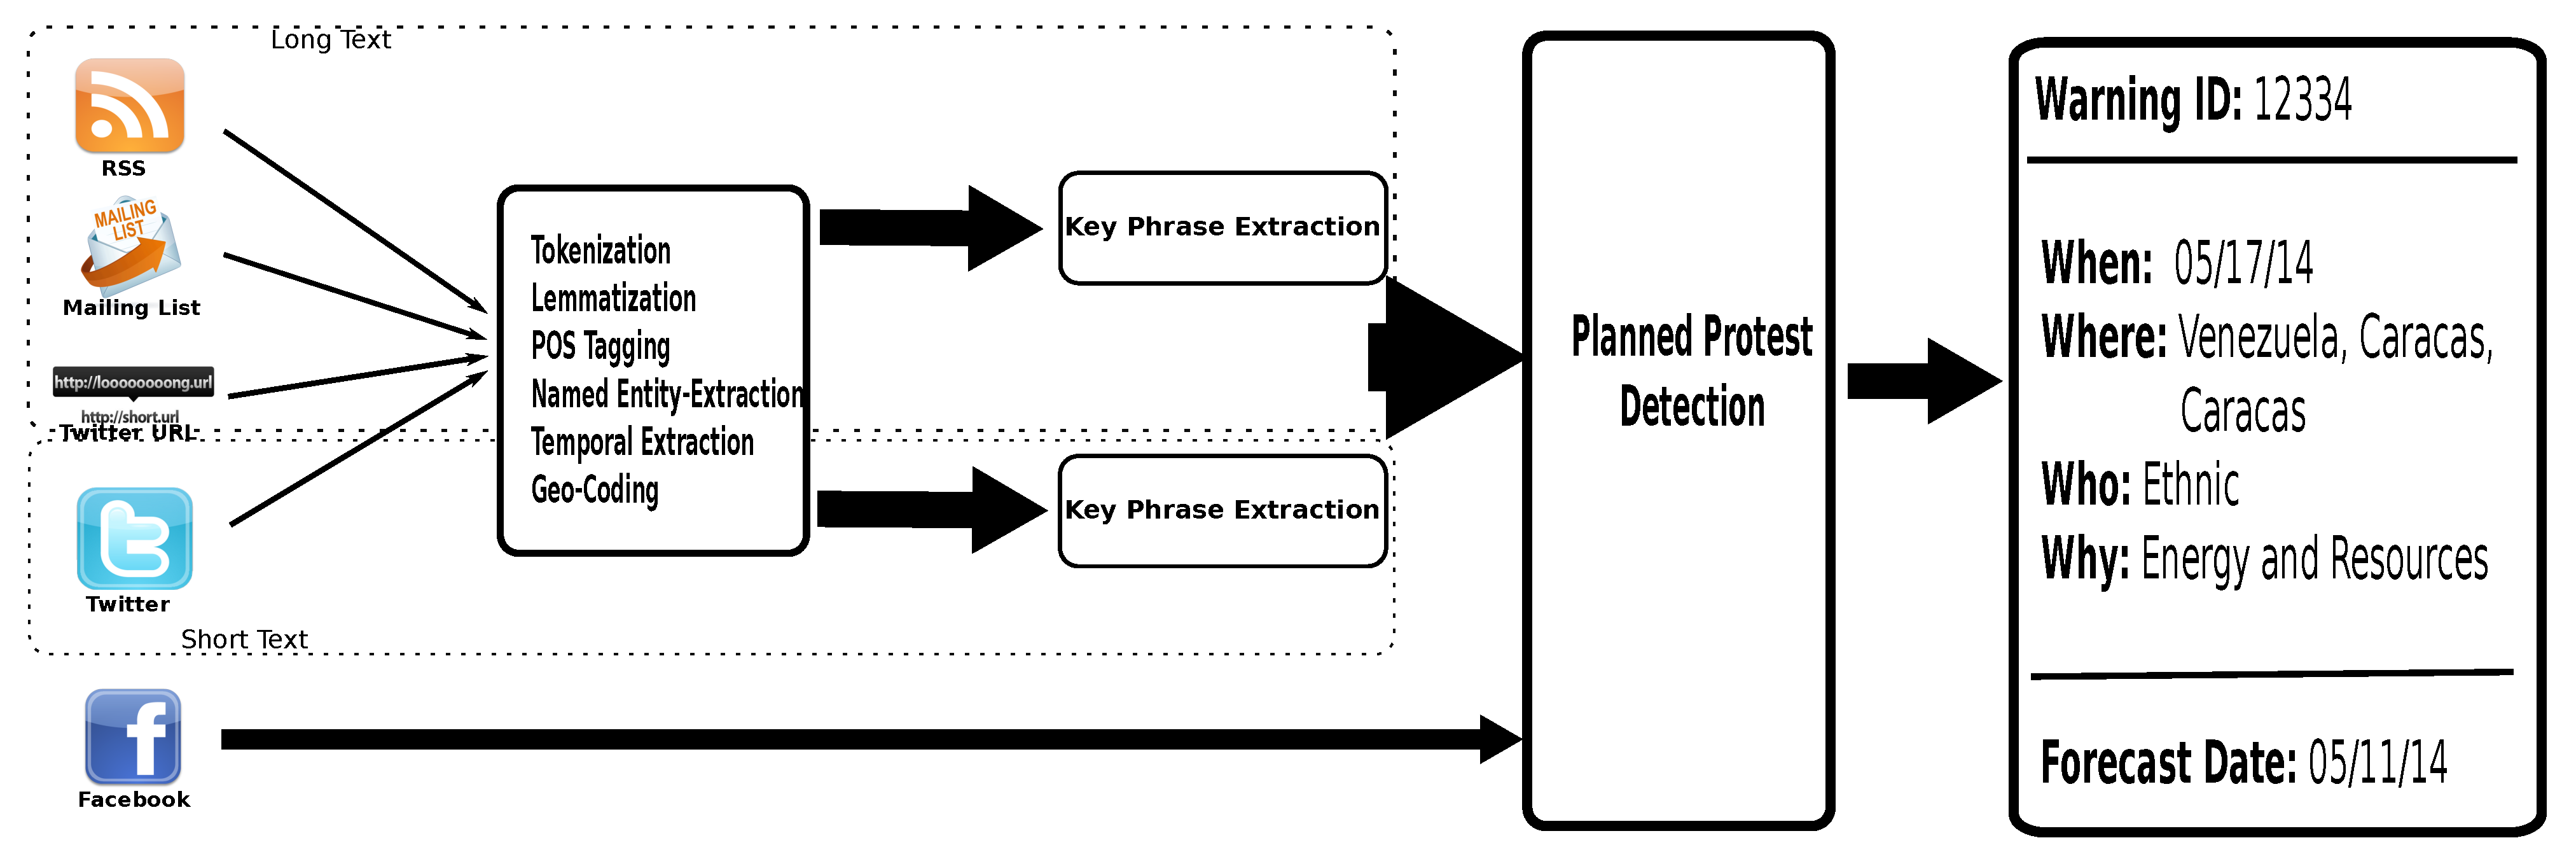
\includegraphics[width=\textwidth]{pp_pipeline}
\caption{A diagram showing various steps of the Model}
\end{figure*}
